\documentclass{article}\usepackage[]{graphicx}\usepackage[]{color}
%% maxwidth is the original width if it is less than linewidth
%% otherwise use linewidth (to make sure the graphics do not exceed the margin)
\makeatletter
\def\maxwidth{ %
  \ifdim\Gin@nat@width>\linewidth
    \linewidth
  \else
    \Gin@nat@width
  \fi
}
\makeatother

\definecolor{fgcolor}{rgb}{0.345, 0.345, 0.345}
\newcommand{\hlnum}[1]{\textcolor[rgb]{0.686,0.059,0.569}{#1}}%
\newcommand{\hlstr}[1]{\textcolor[rgb]{0.192,0.494,0.8}{#1}}%
\newcommand{\hlcom}[1]{\textcolor[rgb]{0.678,0.584,0.686}{\textit{#1}}}%
\newcommand{\hlopt}[1]{\textcolor[rgb]{0,0,0}{#1}}%
\newcommand{\hlstd}[1]{\textcolor[rgb]{0.345,0.345,0.345}{#1}}%
\newcommand{\hlkwa}[1]{\textcolor[rgb]{0.161,0.373,0.58}{\textbf{#1}}}%
\newcommand{\hlkwb}[1]{\textcolor[rgb]{0.69,0.353,0.396}{#1}}%
\newcommand{\hlkwc}[1]{\textcolor[rgb]{0.333,0.667,0.333}{#1}}%
\newcommand{\hlkwd}[1]{\textcolor[rgb]{0.737,0.353,0.396}{\textbf{#1}}}%
\let\hlipl\hlkwb

\usepackage{framed}
\makeatletter
\newenvironment{kframe}{%
 \def\at@end@of@kframe{}%
 \ifinner\ifhmode%
  \def\at@end@of@kframe{\end{minipage}}%
  \begin{minipage}{\columnwidth}%
 \fi\fi%
 \def\FrameCommand##1{\hskip\@totalleftmargin \hskip-\fboxsep
 \colorbox{shadecolor}{##1}\hskip-\fboxsep
     % There is no \\@totalrightmargin, so:
     \hskip-\linewidth \hskip-\@totalleftmargin \hskip\columnwidth}%
 \MakeFramed {\advance\hsize-\width
   \@totalleftmargin\z@ \linewidth\hsize
   \@setminipage}}%
 {\par\unskip\endMakeFramed%
 \at@end@of@kframe}
\makeatother

\definecolor{shadecolor}{rgb}{.97, .97, .97}
\definecolor{messagecolor}{rgb}{0, 0, 0}
\definecolor{warningcolor}{rgb}{1, 0, 1}
\definecolor{errorcolor}{rgb}{1, 0, 0}
\newenvironment{knitrout}{}{} % an empty environment to be redefined in TeX

\usepackage{alltt}
\usepackage{graphicx}
\usepackage{float}
\usepackage{amsmath}
\usepackage{blindtext}
\usepackage[inline]{enumitem}
\usepackage{xcolor}
\usepackage{bm}
\usepackage {fancyvrb}
\usepackage {listings}
\usepackage[makeroom]{cancel}
\usepackage[urlcolor=blue,colorlinks=true]{hyperref}
\IfFileExists{upquote.sty}{\usepackage{upquote}}{}
\begin{document}
Initial coordinates are:

\begin{align*}
  &S\ (0.138,0.0,-1.654)\\
  &C_1\ (0.474, 0.0, 1.059)\\
  &C_2\ (-0.621, 0.0, -0.007)\\
  &O\ (-0.125, 0.0, 2.357)\\
  &H\ (0.598, 0.0, 2.999)
\end{align*}

The axis of rotation is then:

\begin{knitrout}
\definecolor{shadecolor}{rgb}{0.969, 0.969, 0.969}\color{fgcolor}\begin{kframe}
\begin{alltt}
  \hlkwd{library}\hlstd{(scatterplot3d)}
  \hlstd{S} \hlkwb{=} \hlkwd{c}\hlstd{(}\hlnum{0.138}\hlstd{,}\hlnum{0.0}\hlstd{,}\hlopt{-}\hlnum{1.654}\hlstd{)}
  \hlstd{C1} \hlkwb{=} \hlkwd{c}\hlstd{(}\hlnum{0.474}\hlstd{,} \hlnum{0.}\hlstd{,} \hlnum{1.059}\hlstd{)}
  \hlstd{C2} \hlkwb{=} \hlkwd{c}\hlstd{(}\hlopt{-}\hlnum{0.621}\hlstd{,}\hlnum{0.}\hlstd{,}\hlopt{-}\hlnum{0.007}\hlstd{)}
  \hlstd{O} \hlkwb{=} \hlkwd{c}\hlstd{(}\hlopt{-}\hlnum{0.125}\hlstd{,} \hlnum{0.0}\hlstd{,} \hlnum{2.357}\hlstd{)}
  \hlstd{H} \hlkwb{=} \hlkwd{c}\hlstd{(}\hlnum{0.598}\hlstd{,} \hlnum{0.0}\hlstd{,} \hlnum{2.999}\hlstd{)}
  \hlstd{axis} \hlkwb{=} \hlstd{C2}\hlopt{-}\hlstd{C1}
  \hlkwd{message}\hlstd{(}\hlkwd{sprintf}\hlstd{(}\hlstr{"The axis of rotation is: %s"}\hlstd{,}\hlkwd{paste}\hlstd{(axis,}\hlkwc{collapse}\hlstd{=}\hlstr{", "}\hlstd{)))}
\end{alltt}


{\ttfamily\noindent\itshape\color{messagecolor}{\#\# The axis of rotation is: -1.095, 0, -1.066}}\begin{alltt}
  \hlstd{normaxis} \hlkwb{=} \hlstd{axis}\hlopt{/}\hlkwd{sqrt}\hlstd{(}\hlkwd{sum}\hlstd{(axis}\hlopt{^}\hlnum{2}\hlstd{))}
  \hlkwd{message}\hlstd{(}\hlkwd{sprintf}\hlstd{(}\hlstr{"The normed axis of rotation is: %s"}\hlstd{,}\hlkwd{paste}\hlstd{(normaxis,}\hlkwc{collapse} \hlstd{=} \hlstr{", "}\hlstd{)))}
\end{alltt}


{\ttfamily\noindent\itshape\color{messagecolor}{\#\# The normed axis of rotation is: -0.716531434615578, 0, -0.697554803013887}}\begin{alltt}
  \hlcom{#Plot the molecule using scatterplot3d}
  \hlstd{x} \hlkwb{=} \hlkwd{c}\hlstd{(S[}\hlnum{1}\hlstd{],C1[}\hlnum{1}\hlstd{],C2[}\hlnum{1}\hlstd{],O[}\hlnum{1}\hlstd{],H[}\hlnum{1}\hlstd{])}
  \hlstd{y} \hlkwb{=} \hlkwd{c}\hlstd{(S[}\hlnum{2}\hlstd{],C1[}\hlnum{2}\hlstd{],C2[}\hlnum{2}\hlstd{],O[}\hlnum{2}\hlstd{],H[}\hlnum{2}\hlstd{])}
  \hlstd{z} \hlkwb{=} \hlkwd{c}\hlstd{(S[}\hlnum{3}\hlstd{],C1[}\hlnum{3}\hlstd{],C2[}\hlnum{3}\hlstd{],O[}\hlnum{3}\hlstd{],H[}\hlnum{3}\hlstd{])}
  \hlcom{#data_frame = data.frame(x,y,z)}
  \hlkwd{scatterplot3d}\hlstd{(x,y,z,}\hlkwc{type} \hlstd{=} \hlstr{"l"}\hlstd{)}
\end{alltt}
\end{kframe}
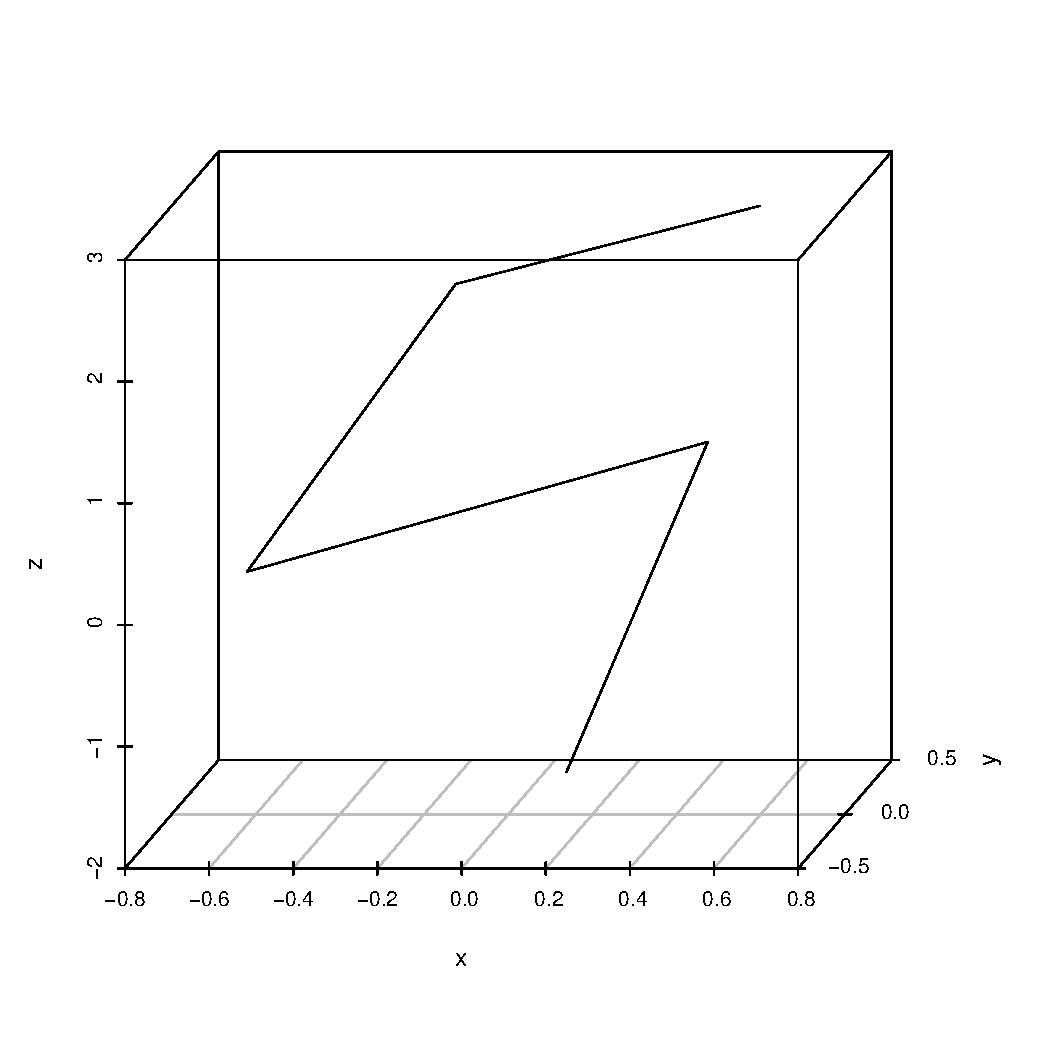
\includegraphics[width=\maxwidth]{figure/define-axis-1} 

\end{knitrout}

The quaternion that defines a $\frac{\pi}{2}$ radian rotation about this axis is:

$$\vec{q}=\cos(\frac{\theta}{2})+\sin(\frac{\theta}{2})\cdot\frac{1}{\| a \|}\vec{a}=\cos(\frac{\pi}{4})+\sin(\frac{\pi}{4})\cdot\frac{1}{\| a \|}\vec{a}$$

This turns out to be:

\begin{knitrout}
\definecolor{shadecolor}{rgb}{0.969, 0.969, 0.969}\color{fgcolor}\begin{kframe}
\begin{alltt}
\hlkwd{library}\hlstd{(onion)}
\hlstd{q} \hlkwb{=} \hlkwd{cos}\hlstd{(pi}\hlopt{/}\hlnum{4}\hlstd{)} \hlopt{+} \hlkwd{sin}\hlstd{(pi}\hlopt{/}\hlnum{4}\hlstd{)} \hlopt{*} \hlstd{normaxis[}\hlnum{1}\hlstd{]} \hlopt{*} \hlstd{Hi} \hlopt{+} \hlkwd{sin}\hlstd{(pi}\hlopt{/}\hlnum{4}\hlstd{)} \hlopt{*} \hlstd{normaxis[}\hlnum{2}\hlstd{]} \hlopt{*} \hlstd{Hj} \hlopt{+}
    \hlkwd{sin}\hlstd{(pi}\hlopt{/}\hlnum{4}\hlstd{)} \hlopt{*} \hlstd{normaxis[}\hlnum{3}\hlstd{]} \hlopt{*} \hlstd{Hk}
\hlkwd{message}\hlstd{(}\hlkwd{sprintf}\hlstd{(}\hlstr{"The quaternion of rotation is %s"}\hlstd{,} \hlkwd{paste}\hlstd{(q,} \hlkwc{collapse} \hlstd{=} \hlstr{", "}\hlstd{)))}
\end{alltt}


{\ttfamily\noindent\itshape\color{messagecolor}{\#\# The quaternion of rotation is 0.707106781186548, -0.50666423635, 0, -0.493245731460365}}\end{kframe}
\end{knitrout}

Finally we get the vectors we wish to rotate:

\begin{knitrout}
\definecolor{shadecolor}{rgb}{0.969, 0.969, 0.969}\color{fgcolor}\begin{kframe}
\begin{alltt}
\hlstd{O} \hlkwb{=} \hlkwd{c}\hlstd{(}\hlopt{-}\hlnum{0.125}\hlstd{,} \hlnum{0}\hlstd{,} \hlnum{2.357}\hlstd{)}
\hlstd{H} \hlkwb{=} \hlkwd{c}\hlstd{(}\hlnum{0.598}\hlstd{,} \hlnum{0}\hlstd{,} \hlnum{2.999}\hlstd{)}
\hlstd{v1} \hlkwb{=} \hlstd{O} \hlopt{-} \hlstd{C2}
\hlstd{v2} \hlkwb{=} \hlstd{H} \hlopt{-} \hlstd{C2}
\hlkwd{message}\hlstd{(}\hlkwd{sprintf}\hlstd{(}\hlstr{"Vector 1 is %s"}\hlstd{,} \hlkwd{paste}\hlstd{(v1,} \hlkwc{collapse} \hlstd{=} \hlstr{", "}\hlstd{)))}
\end{alltt}


{\ttfamily\noindent\itshape\color{messagecolor}{\#\# Vector 1 is 0.496, 0, 2.364}}\begin{alltt}
\hlkwd{message}\hlstd{(}\hlkwd{sprintf}\hlstd{(}\hlstr{"Vector 2 is %s"}\hlstd{,} \hlkwd{paste}\hlstd{(v2,} \hlkwc{collapse} \hlstd{=} \hlstr{", "}\hlstd{)))}
\end{alltt}


{\ttfamily\noindent\itshape\color{messagecolor}{\#\# Vector 2 is 1.219, 0, 3.006}}\end{kframe}
\end{knitrout}

Applying the rotation quaternions we get:

\begin{knitrout}
\definecolor{shadecolor}{rgb}{0.969, 0.969, 0.969}\color{fgcolor}\begin{kframe}
\begin{alltt}
\hlstd{v1_q} \hlkwb{=} \hlnum{0} \hlopt{+} \hlstd{v1[}\hlnum{1}\hlstd{]} \hlopt{*} \hlstd{Hi} \hlopt{+} \hlstd{v1[}\hlnum{2}\hlstd{]} \hlopt{*} \hlstd{Hj} \hlopt{+} \hlstd{v1[}\hlnum{3}\hlstd{]} \hlopt{*} \hlstd{Hk}
\hlstd{v2_q} \hlkwb{=} \hlnum{0} \hlopt{+} \hlstd{v2[}\hlnum{1}\hlstd{]} \hlopt{*} \hlstd{Hi} \hlopt{+} \hlstd{v2[}\hlnum{2}\hlstd{]} \hlopt{*} \hlstd{Hj} \hlopt{+} \hlstd{v2[}\hlnum{3}\hlstd{]} \hlopt{*} \hlstd{Hk}
\hlstd{v1_rot_q} \hlkwb{=} \hlstd{(q} \hlopt{*} \hlstd{v1_q)} \hlopt{*} \hlkwd{Conj}\hlstd{(q)}
\hlstd{v2_rot_q} \hlkwb{=} \hlstd{(q} \hlopt{*} \hlstd{v2_q)} \hlopt{*} \hlkwd{Conj}\hlstd{(q)}
\hlstd{v1_rot} \hlkwb{=} \hlkwd{c}\hlstd{(}\hlkwd{i}\hlstd{(v1_rot_q),} \hlkwd{j}\hlstd{(v1_rot_q),} \hlkwd{k}\hlstd{(v1_rot_q))}
\hlstd{v2_rot} \hlkwb{=} \hlkwd{c}\hlstd{(}\hlkwd{i}\hlstd{(v2_rot_q),} \hlkwd{j}\hlstd{(v2_rot_q),} \hlkwd{k}\hlstd{(v2_rot_q))}
\hlkwd{message}\hlstd{(}\hlkwd{sprintf}\hlstd{(}\hlstr{"v1 rotated pi/2 radians is now %s"}\hlstd{,} \hlkwd{paste}\hlstd{(v1_rot,} \hlkwc{collapse} \hlstd{=} \hlstr{", "}\hlstd{)))}
\end{alltt}


{\ttfamily\noindent\itshape\color{messagecolor}{\#\# v1 rotated pi/2 radians is now 1.43622932617847, 1.34789312913634, 1.39819220247146}}\begin{alltt}
\hlkwd{message}\hlstd{(}\hlkwd{sprintf}\hlstd{(}\hlstr{"v2 rotated pi/2 radians is now %s"}\hlstd{,} \hlkwd{paste}\hlstd{(v2_rot,} \hlkwc{collapse} \hlstd{=} \hlstr{","}\hlstd{)))}
\end{alltt}


{\ttfamily\noindent\itshape\color{messagecolor}{\#\# v2 rotated pi/2 radians is now 2.1283144356317,1.3035741875805,2.07194811724511}}\end{kframe}
\end{knitrout}

This translates to final coordinates of O and H of:

\begin{knitrout}
\definecolor{shadecolor}{rgb}{0.969, 0.969, 0.969}\color{fgcolor}\begin{kframe}
\begin{alltt}
\hlstd{Onew} \hlkwb{=} \hlstd{v1_rot} \hlopt{+} \hlstd{C2}
\hlstd{Hnew} \hlkwb{=} \hlstd{v2_rot} \hlopt{+} \hlstd{C2}
\hlkwd{message}\hlstd{(}\hlkwd{sprintf}\hlstd{(}\hlstr{"Onew is %s"}\hlstd{,} \hlkwd{paste}\hlstd{(Onew,} \hlkwc{collapse} \hlstd{=} \hlstr{", "}\hlstd{)))}
\end{alltt}


{\ttfamily\noindent\itshape\color{messagecolor}{\#\# Onew is 0.815229326178469, 1.34789312913634, 1.39119220247146}}\begin{alltt}
\hlkwd{message}\hlstd{(}\hlkwd{sprintf}\hlstd{(}\hlstr{"Hnew is %s"}\hlstd{,} \hlkwd{paste}\hlstd{(Hnew,} \hlkwc{collapse} \hlstd{=} \hlstr{","}\hlstd{)))}
\end{alltt}


{\ttfamily\noindent\itshape\color{messagecolor}{\#\# Hnew is 1.5073144356317,1.3035741875805,2.06494811724511}}\begin{alltt}
\hlcom{# Plot the new dihedral}
\hlstd{xnew} \hlkwb{=} \hlkwd{c}\hlstd{(S[}\hlnum{1}\hlstd{], C1[}\hlnum{1}\hlstd{], C2[}\hlnum{1}\hlstd{], Onew[}\hlnum{1}\hlstd{], Hnew[}\hlnum{1}\hlstd{])}
\hlstd{ynew} \hlkwb{=} \hlkwd{c}\hlstd{(S[}\hlnum{2}\hlstd{], C1[}\hlnum{2}\hlstd{], C2[}\hlnum{2}\hlstd{], Onew[}\hlnum{2}\hlstd{], Hnew[}\hlnum{2}\hlstd{])}
\hlstd{znew} \hlkwb{=} \hlkwd{c}\hlstd{(S[}\hlnum{3}\hlstd{], C1[}\hlnum{3}\hlstd{], C2[}\hlnum{3}\hlstd{], Onew[}\hlnum{3}\hlstd{], Hnew[}\hlnum{3}\hlstd{])}

\hlstd{xtotal} \hlkwb{=} \hlkwd{c}\hlstd{(x, xnew)}
\hlstd{ytotal} \hlkwb{=} \hlkwd{c}\hlstd{(y, ynew)}
\hlstd{ztotal} \hlkwb{=} \hlkwd{c}\hlstd{(z, znew)}
\hlstd{category} \hlkwb{=} \hlkwd{c}\hlstd{(}\hlkwd{rep}\hlstd{(}\hlstr{"blue"}\hlstd{,} \hlnum{5}\hlstd{),} \hlkwd{rep}\hlstd{(}\hlstr{"red"}\hlstd{,} \hlnum{5}\hlstd{))}
\hlstd{data_frame} \hlkwb{=} \hlkwd{data.frame}\hlstd{(xtotal, ytotal, ztotal)}
\hlstd{data_frame}\hlopt{$}\hlstd{fac} \hlkwb{=} \hlkwd{factor}\hlstd{(}\hlkwd{rep}\hlstd{(LETTERS[}\hlnum{1}\hlopt{:}\hlnum{2}\hlstd{],} \hlkwc{each} \hlstd{=} \hlnum{5}\hlstd{))}
\hlkwd{scatterplot3d}\hlstd{(data_frame}\hlopt{$}\hlstd{xtotal, data_frame}\hlopt{$}\hlstd{ytotal, data_frame}\hlopt{$}\hlstd{ztotal,} \hlkwc{type} \hlstd{=} \hlstr{"l"}\hlstd{,}
    \hlkwc{color} \hlstd{=} \hlkwd{as.numeric}\hlstd{(data_frame}\hlopt{$}\hlstd{fac))}
\end{alltt}
\end{kframe}

\includegraphics[width=\maxwidth]{figure/new-coords-1} 

\end{knitrout}

The calculated dihedral angle from these new coordinates is:

\begin{knitrout}
\definecolor{shadecolor}{rgb}{0.969, 0.969, 0.969}\color{fgcolor}\begin{kframe}
\begin{alltt}
\hlkwd{library}\hlstd{(pracma)}
\end{alltt}


{\ttfamily\noindent\itshape\color{messagecolor}{\#\# \\\#\# Attaching package: 'pracma'}}

{\ttfamily\noindent\itshape\color{messagecolor}{\#\# The following object is masked from 'package:onion':\\\#\# \\\#\#\ \ \ \  Norm}}\begin{alltt}
\hlstd{b1} \hlkwb{=} \hlstd{C1} \hlopt{-} \hlstd{S}
\hlstd{b2} \hlkwb{=} \hlstd{C2} \hlopt{-} \hlstd{C1}
\hlstd{b3} \hlkwb{=} \hlstd{Onew} \hlopt{-} \hlstd{C2}
\hlstd{b2norm} \hlkwb{=} \hlstd{b2}\hlopt{/}\hlkwd{sqrt}\hlstd{(}\hlkwd{sum}\hlstd{(b2}\hlopt{^}\hlnum{2}\hlstd{))}
\hlstd{n1} \hlkwb{=} \hlkwd{cross}\hlstd{(b1, b2)}\hlopt{/}\hlkwd{sqrt}\hlstd{(}\hlkwd{sum}\hlstd{(}\hlkwd{cross}\hlstd{(b1, b2)}\hlopt{^}\hlnum{2}\hlstd{))}
\hlstd{n2} \hlkwb{=} \hlkwd{cross}\hlstd{(b3, b2)}\hlopt{/}\hlkwd{sqrt}\hlstd{(}\hlkwd{sum}\hlstd{(}\hlkwd{cross}\hlstd{(b2, b3)}\hlopt{^}\hlnum{2}\hlstd{))}
\hlstd{m1} \hlkwb{=} \hlkwd{cross}\hlstd{(n1, n2)}
\hlstd{angle} \hlkwb{=} \hlkwd{atan2}\hlstd{((m1} \hlopt \hlstd{b2norm), (n1} \hlopt \hlstd{n2))}
\hlkwd{message}\hlstd{(}\hlkwd{sprintf}\hlstd{(}\hlstr{"The calculated dihedral angle of the resulting rotation is: %4.2f degrees"}\hlstd{,}
    \hlstd{angle} \hlopt{*} \hlnum{180}\hlopt{/}\hlstd{pi))}
\end{alltt}


{\ttfamily\noindent\itshape\color{messagecolor}{\#\# The calculated dihedral angle of the resulting rotation is: 90.00 degrees}}\end{kframe}
\end{knitrout}



\end{document}



















